\documentclass[a4paper,12pt,twoside,openright]{memoir}

\newcommand{\subject}{From Existing Software to Models}

%%%% PACKAGES %%%%

\usepackage[T1]{fontenc}
\usepackage[utf8]{inputenc}
\usepackage{fourier}
\usepackage[english]{babel}

\usepackage{graphicx}
\graphicspath{{Images/}}

\begin{document}

\chapter{Process Analyse}

    \section{Beskrivelse - Hvad gjorde vi i P1} 

        \subsection{Projektplanlægning}

            I hvilket omfang har gruppens medlemmer haft samme opfattelse af hvad projektplanlægning indebærer?\newline

            Opfattelsen af projectplanlægning har i gruppen været hovesaglig, Brainstorm, posters og tidsplanlægning. Hvor alle tre ting kan ændre med tiden. Der blev lavet undervejs to tidsplaner, med deadlines til f.eks. hvornår vi skulle afslutte problemanalysen. Da ikke alle tidspunkter var realistiske under hele forløbet, blev der lavet en ny iteration.\newline

            Har I haft nogle projektplaner? I så fald: Hvilke, hvad har I anvendt dem til og hvordan har de fungeret? Hvis ikke: Vil I lave projektplaner i P1? I så fald: Hvilke og hvad vil I bruge dem til?\newline

            Inden for den første uge af P1, lavede vi en tids plan for P1, tids blev lavet en tidsplan(ses her under) med poster så der let kunne laves om, eller flyttes rundt på emnerne, hvis vi havde brug for mere tid eller hvis et emne blev færdigt. Hen i slutningen af Projektet blev der lavet  en tidsplan v. 2.0. vores arbejde, er blevet udarbejdet  efter tidsplanen, for at kunne have et overblik over hvad der skulle laves og hvornår det skulle være færdigt.

            \begin{figure}[ht!]
                \centering
                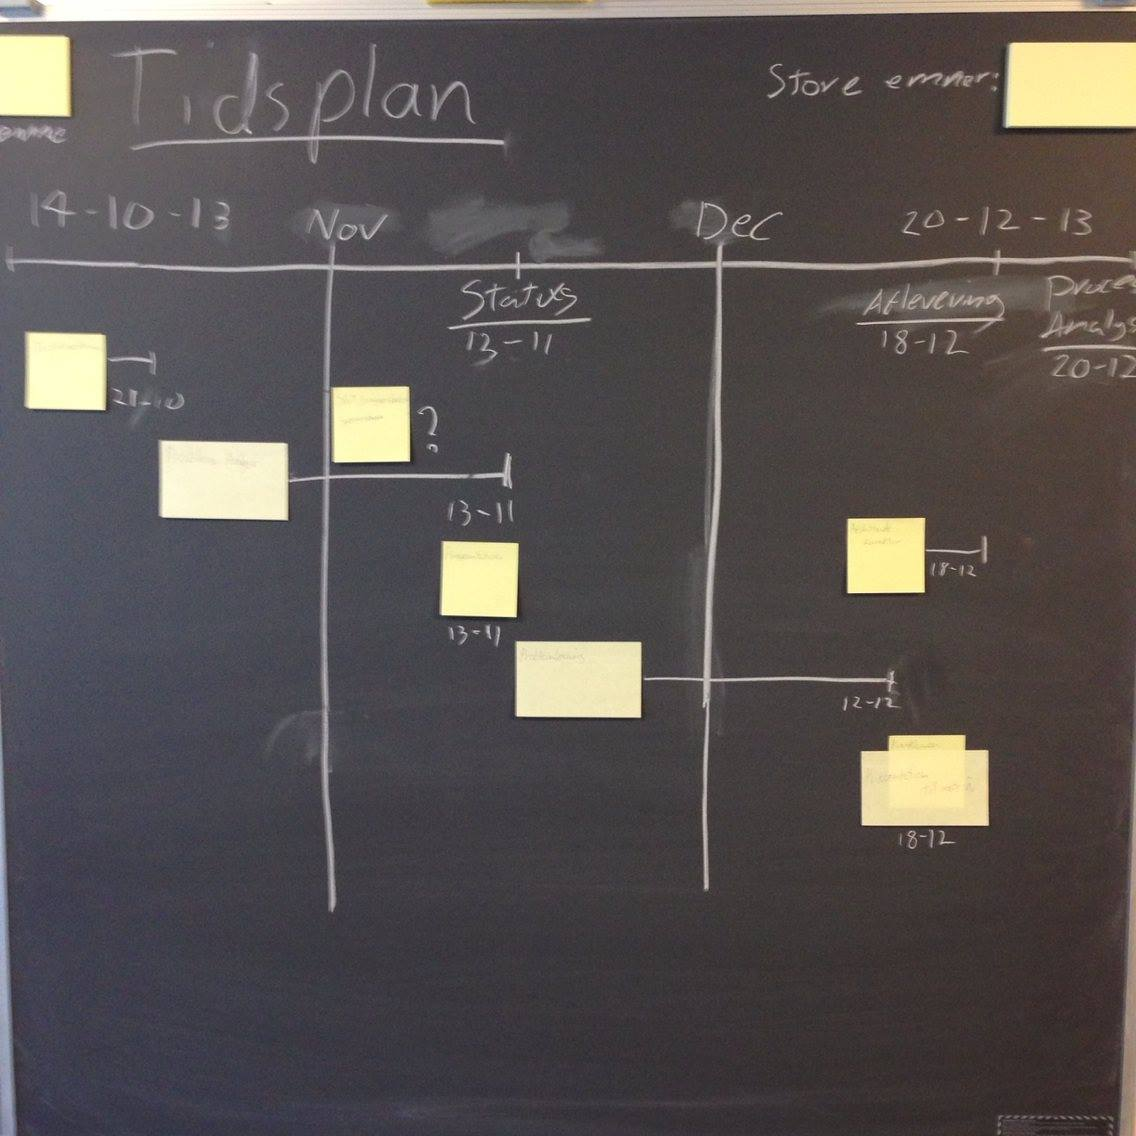
\includegraphics[width=0.5\textwidth]{Images/9.jpg}
                \caption{BAH}
                \label{4}
            \end{figure}

            \begin{figure}[ht!]
                \centering
                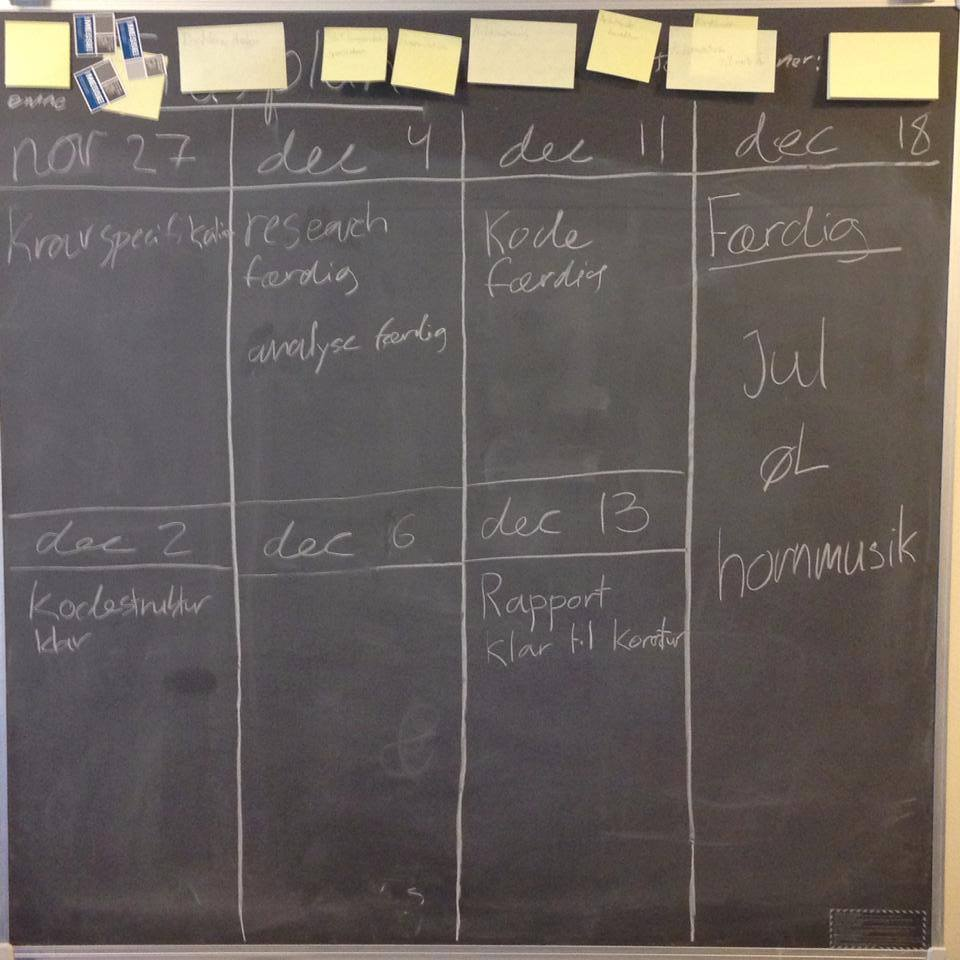
\includegraphics[width=0.5\textwidth]{Images/2.jpg}
                \caption{BAH}
                \label{4}
            \end{figure}

        \subsection{Gruppesamarbejde}
            
            Gruppen har været enige om et ambitionsniveau, og der været en generel deltagelse i sociale aktiviteter. En fælles samarbejdsaftale blev lavet, med aftaler om mødetider og regler omkring brug af software.

            Har I lavet en samarbejdsaftale (mundtlig/skriftlig)? Hvorfor/Hvorfor ikke? 
            
            Hvor tit har I holdt møder?  
            Hvad gjorde I hvis en person kom for sent/ikke kom til møderne? 
            Hvordan har I afviklet møderne? (F.eks. med mødeleder, via runder om bordet, fri diskussion etc.) 
            Hvordan har kommunikationen været i jeres gruppe? Var der nogen, der talte hele tiden? Var der nogen, der aldrig sagde noget? Brugte gruppen uforholdsvis lang tid på diskussioner? Hvorfor? 
            Hvordan har motivationen været hos de enkelte gruppemedlemmer? Har I oplevet problemer med forskelle i motivation? I så fald: Hvad har I gjort for at løse problemerne? 
            Efter hvilke kriterier har I fordelt arbejdsopgaverne mellem jer? Har det fungeret tilfredsstillende for alle? 
            Hvordan sikrede I konstruktiv kritik af hinandens arbejdsblade til rapporten? 



            Vores gruppe har primært arbejdet i små gruppere, fordi vi mener at for mange på en opgave ikke nødvendigvis giver bedre resultat og da gruppen regelmæssig diskutere om forskellige emner, har det været en god ide at lave så grupper så en diskussion ikke har stoppet alt arbejdet, men alt har været snakket igennem i gruppen, selvom vi har arbejdet i mindre grupper. 

            Når vi har valgt at arbejde i små grupper, har vi også været ude for at skulle diskutere noget, diskussion har startet i den lille gruppe er blevet diskuteret vidre i hele gruppen så alle er kommet med input og de positive og negative sider og blevet vendt.

            I gruppen har vi under projekt arbejde og materiale søgning, arbejdet i små grupper, hvor vi har arbejdet ud fra belbin arbejds model, hvor vi har laveet  gruppen så mindst et medlem har stor viden inden for emnet eller programering, så denne person kunne forklarer og vise hvordan han har løst opgaven. 
            Når vi har lavet grupper og fordelt arbejdet, har vi sat nogle emner op på det der skal laves og folk har kunne vælge dem de ville arbejde med og dermed delt os i små grupper, så vi har kunne lave flere ting på en gang, men hver dag har vi lavet gruppe møde på hvad der er blevet laver  og hvor langt de enkelte grupper er. Efter gruppe arbejde har vi snakket om det i hele gruppen, og givet  hinanden kontroktiv kritik.

            \begin{figure}[ht!]
                \centering
                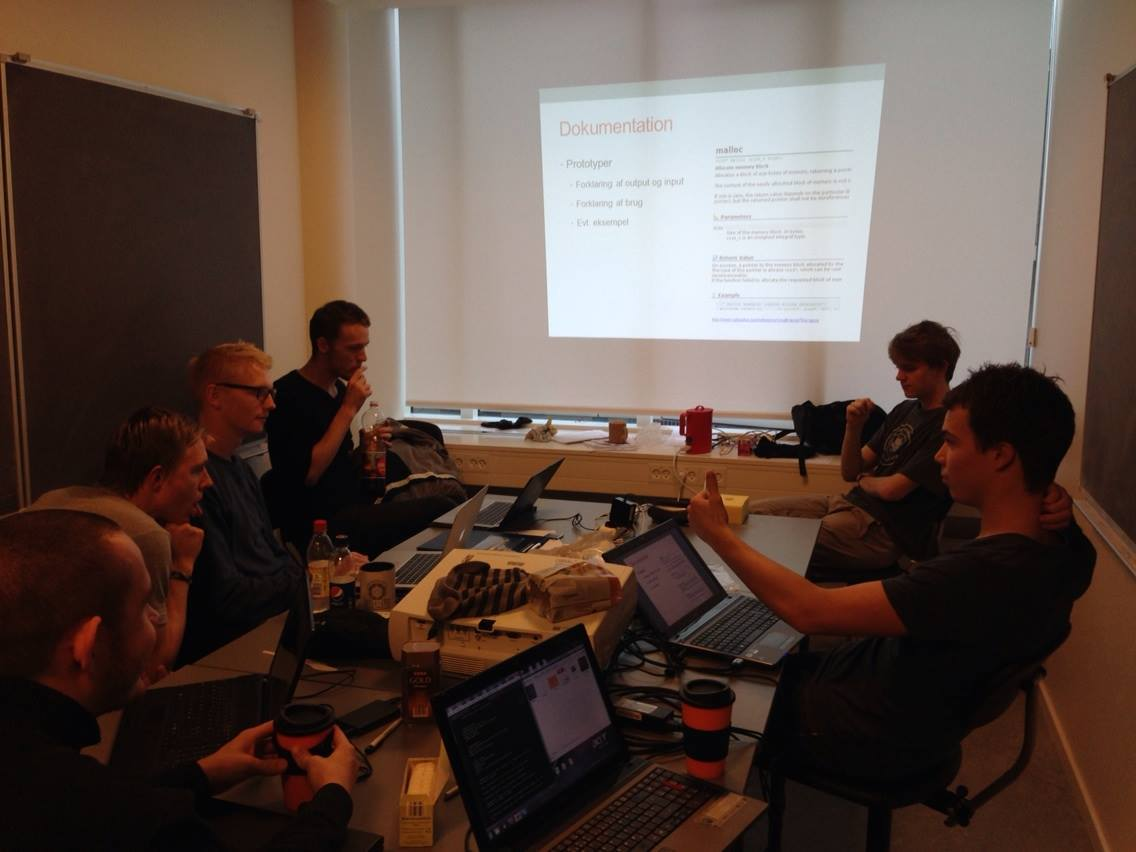
\includegraphics[width=0.5\textwidth]{Images/8.jpg}
                \caption{BAH}
                \label{4}
            \end{figure}

        \subsection{Samarbejde med vejlederen}
        % Har I haft en samarbejdsaftale med jeres vejleder? I så fald: har den fungeret tilfredsstillende? 
        % Hvordan forberedte I møder med jeres vejleder? 
        % Hvilken type vejledning ønskede I fra vejlederen? Hvilken type vejledning fik I?


Ja, ved første møde med vejlederen, blev vejleder samarbejdsaftalen introduceret. Aftalen bestod af 7 punkter. Samarbejdsaftalen har fungeret fint som en base for samarbejdet mellem gruppen og vejlederen, så den kan fint siges at have fungeret tilfredsstillende. Møder med vejlederen blev typisk forberedt så sent som muligt, således at de seneste problemer/spørgsmål kunne komme med i dagsordenen. Forberedelsen foregik ved at en computer blev tilsluttet en projektor, hvorefter gruppens medlemmer kunne komme med input til dagsordenen. Dette kunne f.eks. være spørgsmål til vejlederen. Disse møder blev holdt med ca. en uges mellemrum, eller aftalt efter deadlines osv.

Den ønskede vejledning fra vejlederen var typisk spørgsmål omkring struktur, f.eks. hvad forskellige dele af rapporten skal indeholde. Ellers blev vejlederen brugt, specielt i rapportens afslutning, til at få respons på de arbejdsark der blev sendt minimum 24 timer før mødet.

        \subsection{Problemformuleringer}
        Hvordan lavede I indledning til problemformuleringen?
        Hvilken argumentation brugte I for at motivere problemformuleringen?
        Hvad har I lært om hvordan problemformuleringer udarbejdes?

        \subsection{Rapportstrukturering}
        Hvordan bestemte I hvilke afsnit der skulle være i jeres P0 rapport?
        Hvordan bestemte I strukturen i rapporten?
        Hvordan sikrede I en rød tråd i rapporten?
        Hvilke afsnit havde I i jeres rapport, som I mener er generelle for alle projekter?

    \section{Vurdering - Hvordan gik det}
    Når I er færdige med at beskrive hvad I gjorde, skal I vurdere hvordan det gik. Med andre ord: Hvad gik godt i P0? Hvad gik dårligt i P0? 

    \section{Analyse - Hvorfor gik det som det gik}
    Dernæst skal I analysere jeres arbejdsprocesser og få klarlagt hvorfor noget gik godt mens andet gik dårligt. Med andre ord: Hvad er det for faktorer, som har indvirket på arbejdsprocesserne? 

        \subsection{Brainstorm}
        I starten af forløbet, lavede i brainstorm på tavlen, hvor vi delte det op i 3 store  emner, "Indoor navigation", "Problemer der skal håndteres" og "Intressenter". Disse emner blev delt ind i under emner, hvor vi smed relevante problemer og emner op omkring navigation eller SOTA som kan buges til navigation. 

        \begin{figure}
        \centering
            \begin{minipage}{0.45\textwidth}
                \centering
                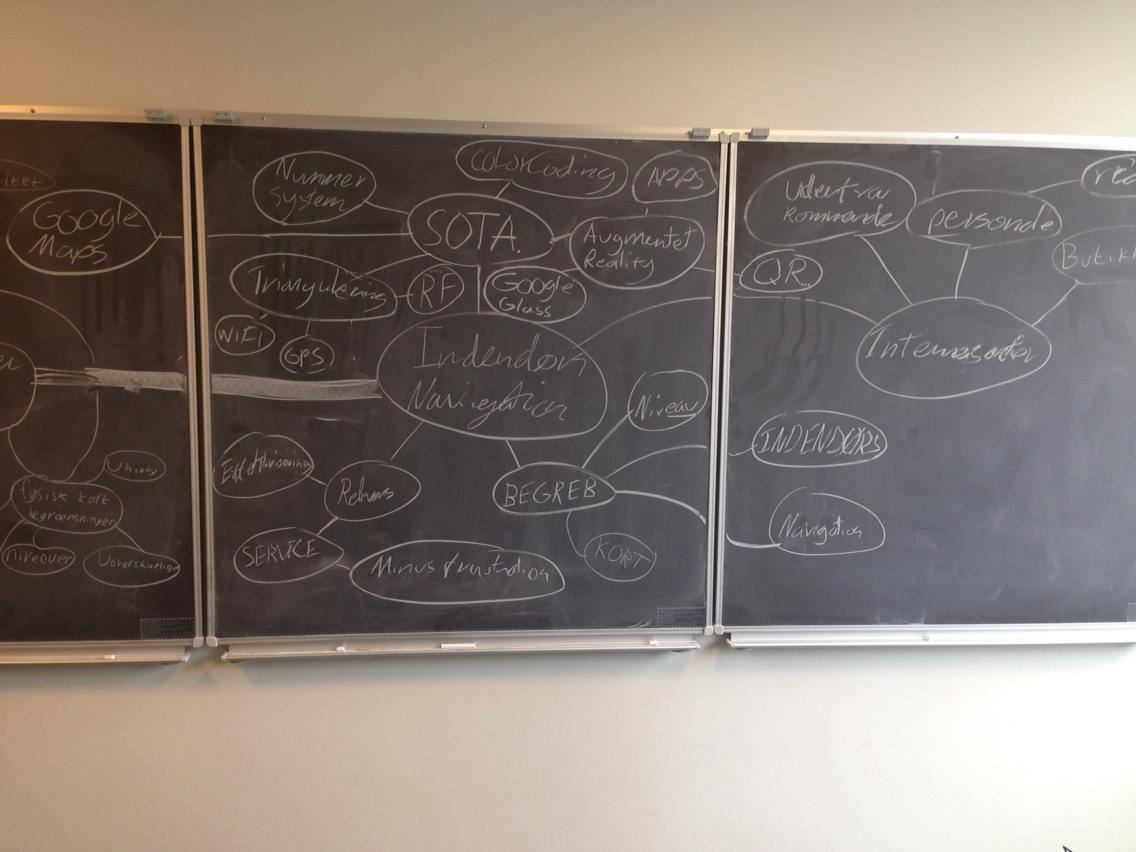
\includegraphics[width=\textwidth]{Images/1.jpg}
                \caption{BAH}
                \label{4}
            \end{minipage}
            \begin{minipage}{0.45\textwidth}
                \centering
                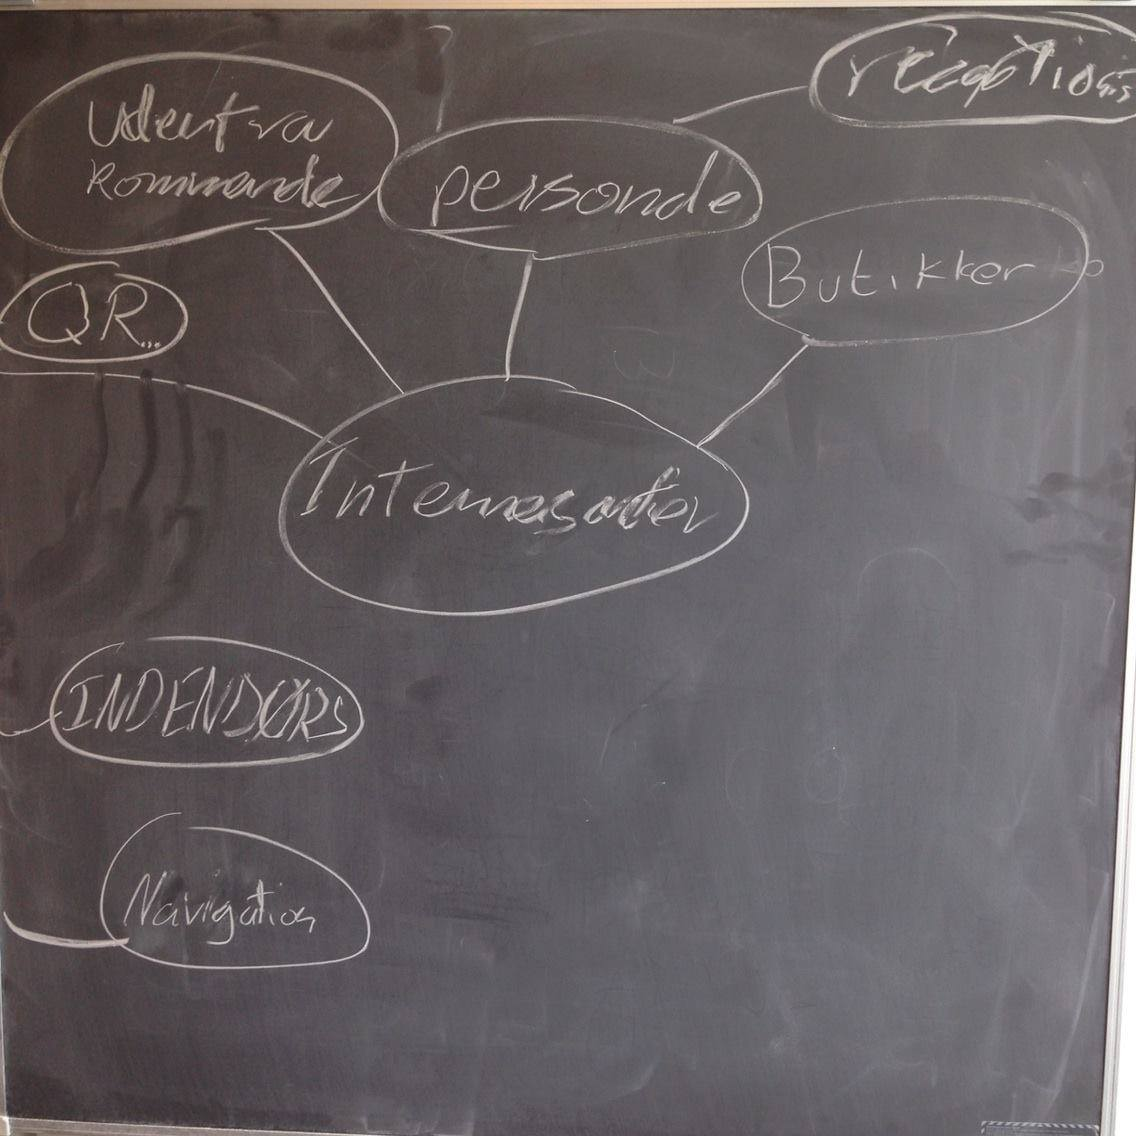
\includegraphics[width=\textwidth]{Images/3.jpg}
                \caption{BAH}
                \label{4}
            \end{minipage}
            \begin{minipage}{0.45\textwidth}
                \centering
                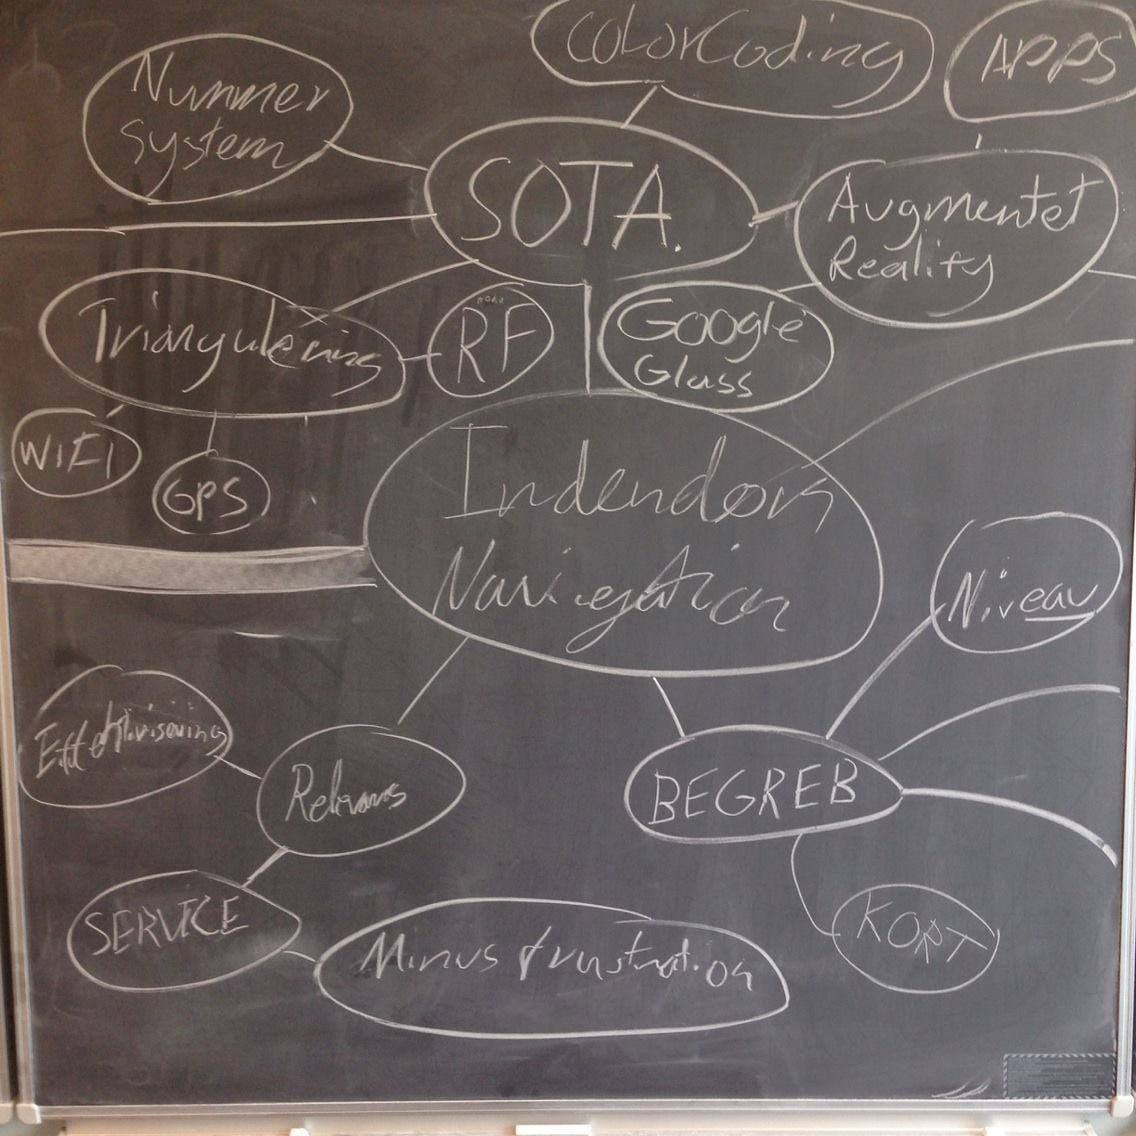
\includegraphics[width=\textwidth]{Images/4.jpg}
                \caption{BAH}
                \label{4}
            \end{minipage}
            \begin{minipage}{0.45\textwidth}
                \centering
                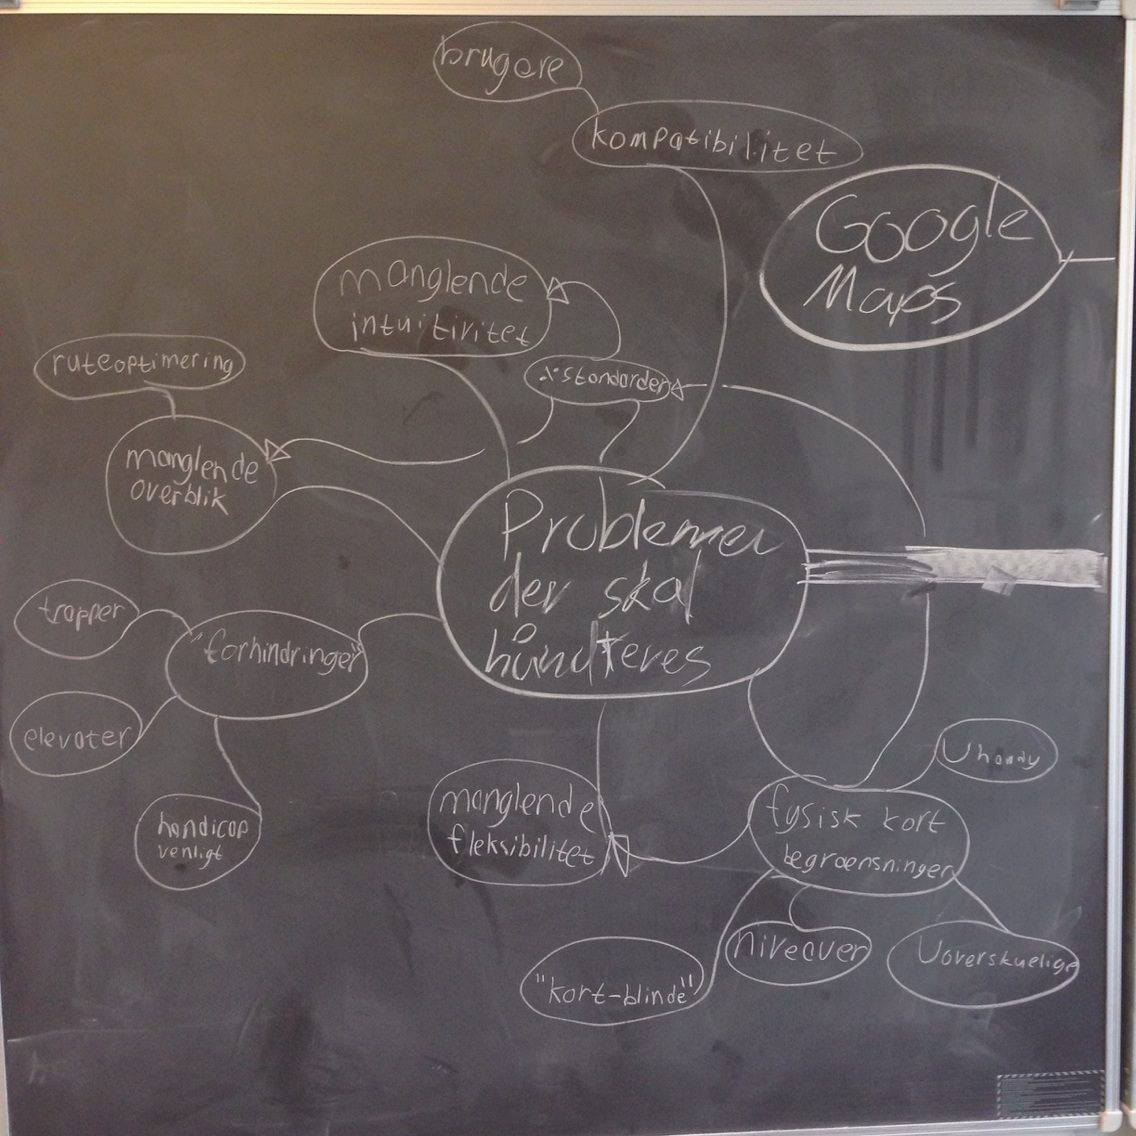
\includegraphics[width=\textwidth]{Images/7.jpg}
                \caption{BAH}
                \label{4}
            \end{minipage}
        \end{figure}

        \subsection{Tegninger}
        Under mange af vores diskussioner, har vi illustreret det for gruppen på tavlen, så alle kunne være  med og her er et af ex. på vores diskussion omkring håndtering af "Floors", der er blevet lavet mange gode ting på tavlen, men ikke alle ting er der blevet taget billeder af.

        \begin{figure}[ht!]
            \centering
            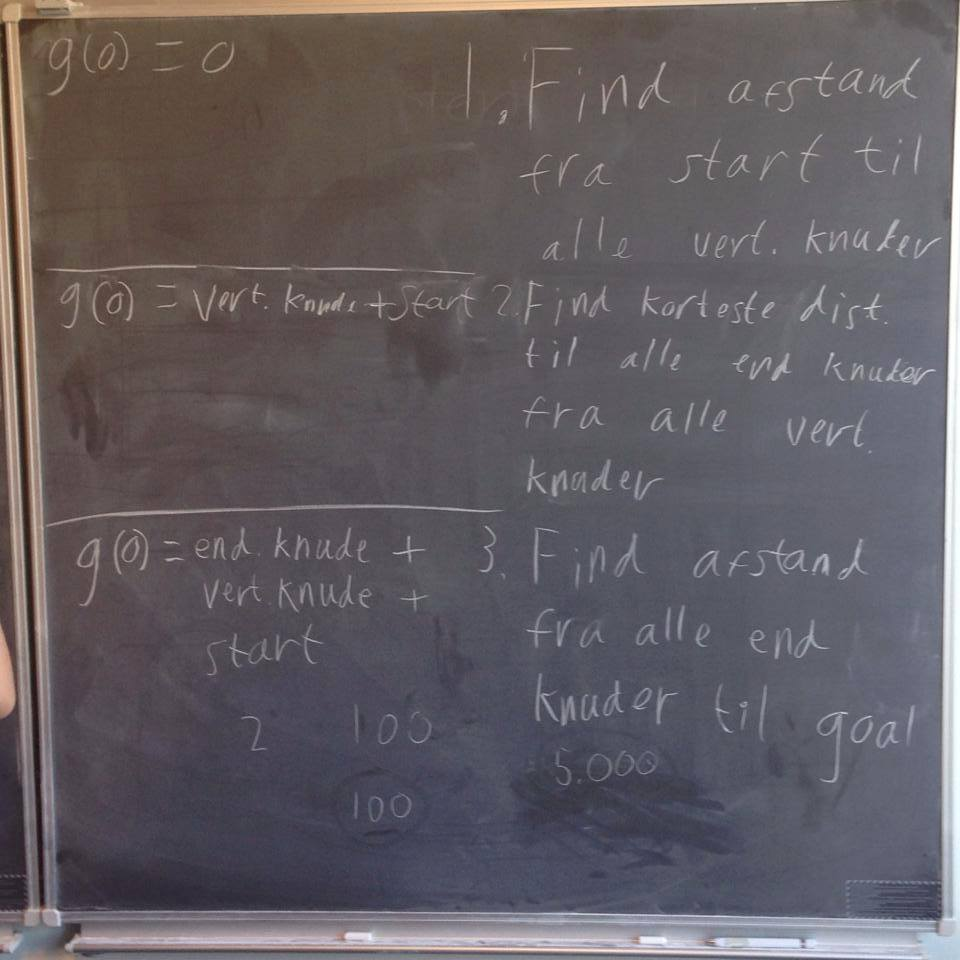
\includegraphics[width=0.5\textwidth]{Images/5.jpg}
            \caption{BAH}
            \label{4}
        \end{figure}

        \begin{figure}[ht!]
            \centering
            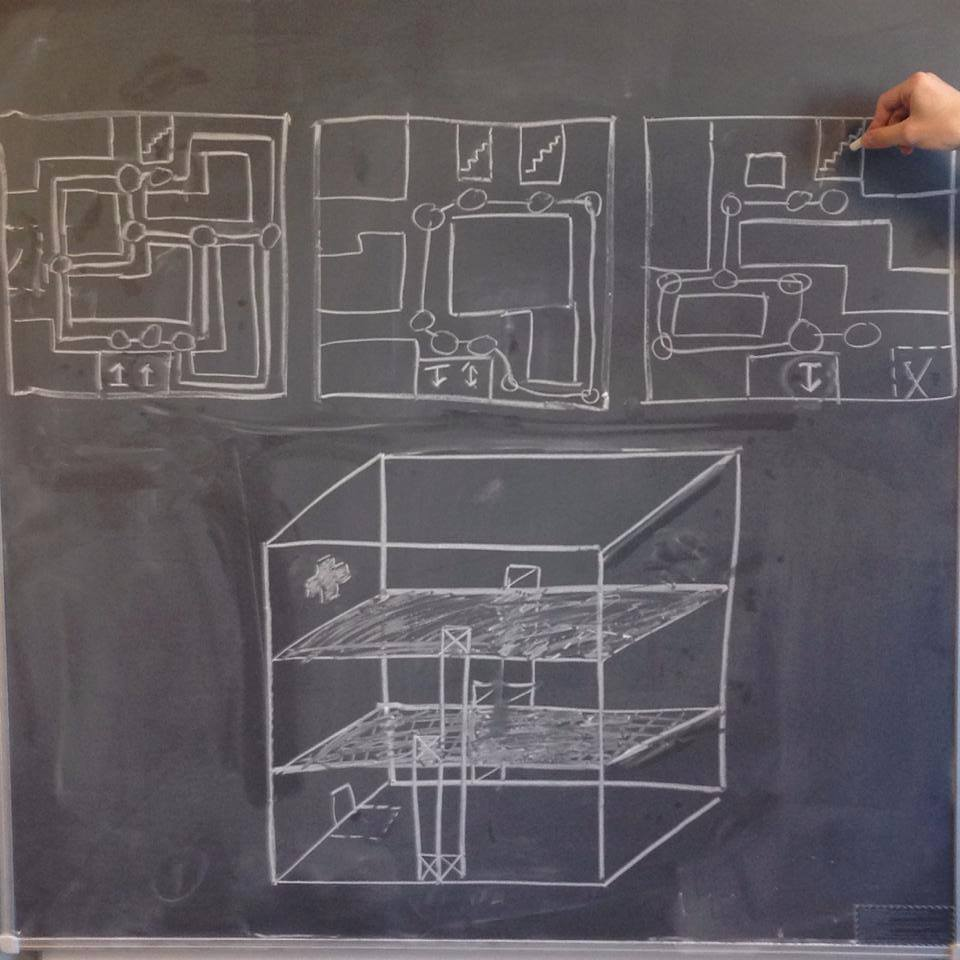
\includegraphics[width=0.5\textwidth]{Images/6.jpg}
            \caption{BAH}
            \label{4}
        \end{figure}

        \subsection{Andet}
        Under materialle læsning, sendte vi en gruppe ud på Syghus Nord Aalborg, for at tage billeder af hvordan navigeringen foregik, såsom farve kode, kort og skilte.

        Der har ikke været en person, der blev udpeget at været projektleder, istedet har vi været meget demokratiske. Tilsidst i projekt forløbet tog nogle gruppemedlem rollen, som projektleder for en dag, hvis rolle var at skulle styr på hvad der var lavet og hvad der stadig manglede at blivet lavet. Beslutninger har været mere enstemmige, men beslutningerne har også først været taget efter længere diskussioner.

    \section{Syntese - Gode råd til P2}
    Hvis jeres vurdering og analyse skal bidrage til at forbedre jeres evne til at håndtere det 
    problemorienterede og projektorganiserede gruppearbejde, skal I til slut konkretisere jeres 
    erfaringer i nogle ’Gode råd’ til jer selv og jeres medstuderende. En god måde at formulere sådanne 
    gode råd på er som en *start-stop-fortsæt*-liste, dvs. en liste med følgende tre sektioner: 
    Dette vil vi begynde at gøre i P1, som vi ikke gjorde i P0 
    Dette vil vi ikke gøre i P1, som vi gjorde i P0 
    Dette vil vi fortsætte med at gøre (gerne anderledes og bedre) i P1, som vi også gjorde i P0 

\end{document}